\par A interação eletromagnética de radiação com a matéria condensada é uma das áreas mais estudadas na física do estado sólido. Sabe-se que a radiação eletromagnética é composta de pequenos pacotes de energia, os fótons\cite{bulk2}. 

\par Devido ao caráter discreto dos níveis de energia dos elétrons e buracos do nosso sistema, a absorção do fóton pode ocorrer através de diferentes mecanismos dependendo da faixa de energia do fóton incidente. De modo geral a transição eletrônica causada pelos fótons absorvidos pode ser dividida em transição interbanda e transição intrabanda\cite{bulk2}.

A transição intrabanda ocorre somente entre os estados presentes dentro da banda de valência ou de condução. Neste caso, a energia incidente dos fótons é muito baixa, onde os comprimentos de onda são grandes (espectro próximo ao infravermelho). Já no caso das transições interbandas, as transições ocorrem entre a banda de condução e a banda de valência, seus valores são consideravelmente maiores que os da transição intrabanda e são somente possíveis quando a energia do fóton incidente é maior que a energia do gap de energia do material \cite{bulk2}. Estas duas formas de transição estão melhores representadas na figura abaixo. 

\begin{figure}[H]
  \centering
  \caption{Diferentes tipos de absorção de fóton para uma fonte de energia $E=\hbar \omega$, a esquerda ocorre interação intrabanda e a direita interação interbanda\cite{bulk2}.}
  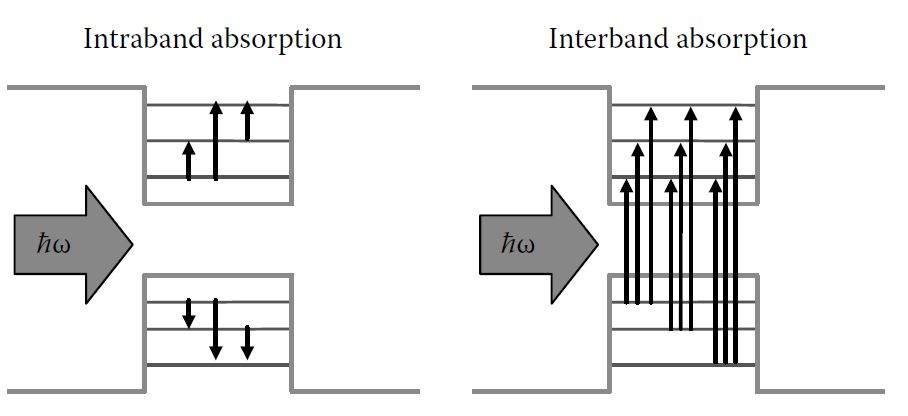
\includegraphics[width=0.65\textwidth]{images/figura16.jpg}
  \label{fig16}
\end{figure}


Nos materiais semicondutores, quando o elétron volta a seu estado original ele pode emitir a energia do éxciton na forma de radiação eletromagnética, efeito conhecido como fluorescência. A criação do éxciton em um ponto quântico tem um raio de éxciton de Bohr consideravelmente menor que o tamanho do ponto quântico em si, como já fora visto anteriormente, caracterizando um confinamento quântico. \cite{optica1}\cite{bulk2}. As propriedades ópticas dos pontos quânticos ocorrem devido ao efeito de confinamento e a equação de Brus apresenta um modelo quantitativo do efeito de confinamento em partículas semicondutoras. A relação abaixo é obtida através da equação de Brus relaciona a energia de transição e com o tamanho do ponto quântico:

\begin{equation}
	\label{optica_1}
	\Delta E(R) = E_{g} + \frac{h^2}{8R^2} \left(\frac{1}{m^{\ast}_{e}} + \frac{1}{m^{\ast}_{h}} \right) - \frac{1.8e^2}{4\pi \epsilon_{b} \epsilon{0}R}
\end{equation}
onde $\Delta E(R)$ é a energia de transição e $E_{g}$, o \textit{gap} da banda do material \textit{bulk}

A equação acima é um modelo relativamente simples com diversas limitações, mas apesar disso, permite analisar a magnitude de energia do confinamento\cite{optica2}\cite{bulk2}. Deste modo a energia de transição também pode ser escrita como:

\begin{equation}
	\label{optica_2}
	\Delta E = \frac{hc}{\lambda}
\end{equation}
onde $c$ é a velocidade da luz no vácuo $(3\cdot 10^8 m/s)$ e $\lambda$ é o comprimento de onda.

Assim, é possível relacionar o tamanho do ponto quântico com o comprimento de onda emitido quando ele for excitado. Observa-se das equações \eqref{optica_1} e \eqref{optica_2} acima  que  o gap de energia fica maior conforme se diminui o tamanho da partícula. Isso justifica o comprimento de onda azul, que é mais energético, ser emitido por partículas de menor diâmetro. Partículas de maior diâmetro exibirão cores no espectro visível associadas a maiores comprimentos de onda, que são menos energéticos. O efeito do tamanho do ponto sobre o comprimento de onda emitido pode ser melhor observado na figura abaixo. 

\begin{figure}[H]
  \centering
  \caption{Estrutura eletrônica variando de acordo com o tamanho do ponto quântico\cite{optica1}.}
  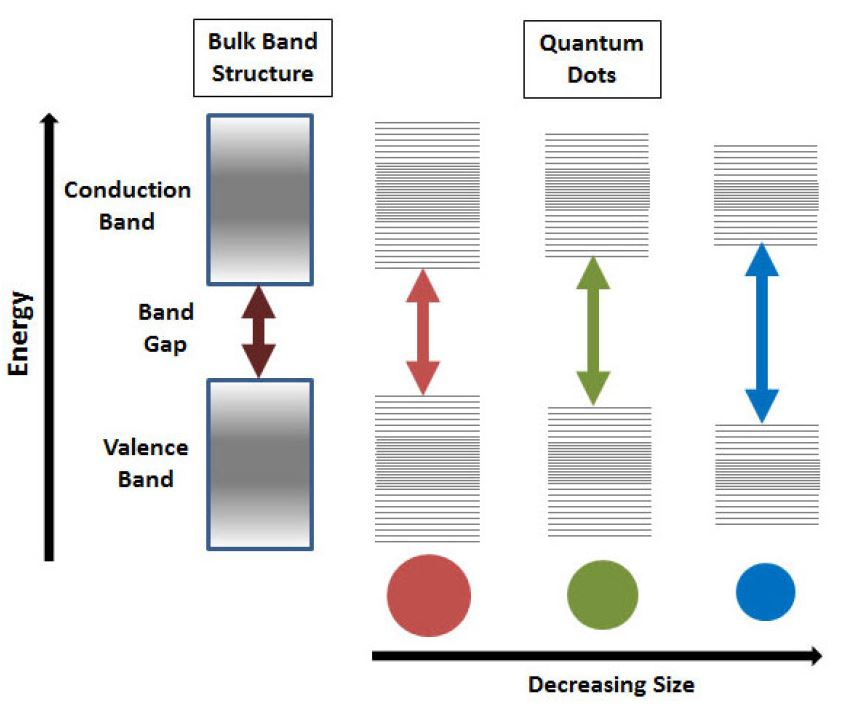
\includegraphics[width=0.65\textwidth]{images/figura17.jpg}
  \label{fig17}
\end{figure}